\documentclass[11pt]{article}

\usepackage[letterpaper,margin=1.0in]{geometry}
\usepackage[T1]{fontenc}
\usepackage{lmodern}
\usepackage{graphicx}
\usepackage{booktabs}
\usepackage{array}
\usepackage{amsmath}
\usepackage{amssymb}
\usepackage{xcolor}
\usepackage[font=small,labelfont=bf]{caption}
\usepackage{enumitem}
\usepackage[round]{natbib}
\usepackage{titlesec}
\usepackage{float}
\usepackage[colorlinks=true,linkcolor=black,citecolor=black,urlcolor=blue]{hyperref}

\titlespacing*{\section}{0pt}{2.2ex plus 0.6ex minus 0.2ex}{1.4ex}
\titlespacing*{\subsection}{0pt}{1.9ex plus 0.5ex minus 0.2ex}{1.0ex}
\setlength{\parskip}{0pt}

\setcounter{topnumber}{2}
\renewcommand{\topfraction}{0.92}
\renewcommand{\textfraction}{0.08}
\renewcommand{\floatpagefraction}{0.85}
\captionsetup[table]{skip=4pt}
\bibliographystyle{plainnat}


\title{\vspace{-2.5em}Does Model Compression Undo Robustness?\\
\large Group robustness of compressed vision transformers,\\
and whether data pruning survives deployment}

\author{Shreyas Visweshwaran \and Swasti Sadanand \and Anusha Upadhyay}
\date{CSC 591/791, ECE 591: Deep Learning Beyond Accuracy\\North Carolina
State University}

\begin{document}
\maketitle
\vspace{-1.5em}

\begin{abstract}
\noindent
We fine-tuned a ViT-S/16 on Waterbirds, compressed it four ways, and looked at
what each compression setting did to the four groups separately. Pruning 30\%
of the transformer weights costs 0.5 points of adjusted average accuracy and
14.9 points on the worst group, a ratio of 29 to one, so a reviewer watching
only the average would have signed this model off. We then repaired the model
with the data pruning of \citet{mulchandani2025severing} and ran the identical
sweep on the repaired checkpoint. The repair gives back 13.9 points on average
across nine arms and 14.6 at its best budget. It also survives compression:
measuring what is left with a retention ratio $R$, we find $R \geq 0.75$ in
95\% of the 87 compressed settings where the model still works at all, and
almost nothing that distinguishes one compression family from another. Where
$R$ goes negative the repair has usually not been destroyed. It is still worth
21.9 points to the group it was aimed at, and worst-group accuracy has quietly
moved to a different group.
\end{abstract}

\section{Introduction}

A model that has been made robust is usually made small afterwards, and the
second step is checked less carefully than the first. The usual check is top-1
accuracy before and after. An average cannot show that one small group has
been abandoned, and it is exactly a small group that a robustness fix buys.
If compression takes the fix back, the average stays quiet.

We work on Waterbirds \citep{sagawa2020distributionally}, where the background
predicts the label for 95\% of the training set, and on a ViT-S/16
\citep{dosovitskiy2021image}. Phase 1 fine-tunes with no group-aware
machinery, compresses that checkpoint four ways and records per-group accuracy
at all 29 settings. Phase 2 repairs the model first, then runs the same sweep.

Four things come out of this. Compression damage is group-asymmetric on a
transformer, and at 30\% sparsity the worst group falls 29 times faster than
the adjusted average. The identifiable-setting rule of
\citet{mulchandani2025severing} reproduces on a different backbone at a tenth
of the schedule and with group-blind selection, recovering 14.6 of their 16.1
points. The retention ratio we use comes with two cases where we refuse to
report it rather than print a number we do not believe. And retention depends
on whether the compressed model still works, not on how it was compressed,
which is not what we expected.

\section{Related work}

\citet{sagawa2020distributionally} introduced Waterbirds and the worst-group
convention, and \citet{koh2021wilds} folded it into WILDS with the adjusted
average. Both evaluate the model at the size it was trained.

\citet{mulchandani2025severing} argue that a spurious correlation is learned
because of a few training samples whose core feature is hard, so deleting
those samples removes the incentive to take the shortcut. On Waterbirds, which
they call an identifiable setting, the rule uses group labels and draws
deletion candidates only from the spurious-aligned group of each class. We
reproduce that rule and treat the result as the thing to compress.

Our four compression families are each well studied on their own, with the
references in Section~\ref{sec:background}. \citet{hooker2019forget} found
that pruned CNNs concentrate their new errors on atypical examples, and
\citet{hooker2020bias} tied that to demographic subgroups on CelebA. We differ
from them on two counts: the backbone is a transformer, and the disparity we
watch was installed by us a few hours earlier rather than inherited from the
data.

\section{Background and problem description} \label{sec:background}

ViT-S/16 \citep{dosovitskiy2021image} cuts a $224 \times 224$ image into
$16 \times 16$ patches and runs them through 12 blocks. Each block has 6
attention heads of width 64 over a 384-channel embedding and an MLP that
widens 384 to 1536 and back, so there are 72 heads to prune from. Magnitude pruning \citep{han2015learning} zeroes the smallest weights and
leaves tensor shapes alone. Head and neuron removal \citep{michel2019sixteen}
deletes whole units, so the zeros arrive in blocks. Quantization
\citep{krishnamoorthi2018quantizing} keeps every weight at lower precision,
the scale set per matrix or per output row;
\citet{krishnamoorthi2018quantizing} showed how much the finer scale recovers.

Waterbirds pastes cropped birds onto Places \citep{zhou2018places}
backgrounds. We read the official splits from \texttt{metadata.csv}: 4795
training images, 1199 validation and 5794 test. A group is $g = 2y + b$ for
label $y$ and background $b$, giving landbird-on-land (3498 training images),
landbird-on-water (184), waterbird-on-land (56) and waterbird-on-water (1057),
written g0 to g3. The two middle groups contradict the shortcut, and g2, with
56 training images, is the worst group almost everywhere below. The test split
is far more group-balanced than the training split, so a plain test mean is
not comparable to published Waterbirds numbers. We follow WILDS and report the
adjusted average, which reweights per-group accuracy by training frequency.

Three choices decide what we are measuring. Training is group-blind, with no
reweighting, no balanced sampler and no robust objective, because a model that
never learned the shortcut leaves nothing for compression to damage. Selection is on plain validation accuracy. The config key is still named
\texttt{select\_on: val\_acc\_avg}, which is misleading: the code reads
\texttt{acc\_avg\_plain}, and selecting on the worst group would be a
group-aware intervention in a run meant to have none. Nothing is
retrained after compression, which would let the network refit the shortcut.

With $W(s)$ the worst-group accuracy and $A(s)$ the adjusted average at
setting $s$, Phase 1 asks whether $W$ falls faster than $A$. Phase 2 trains a
model whose $W$ starts higher and asks how much of the head start is left.

\section{Method}

\subsection{A frozen compression scope}

Four families are only comparable if they may touch the same parameters, so we
fixed the scope once and never moved it: the in-block linear weights
\texttt{attn.qkv}, \texttt{attn.proj}, \texttt{mlp.fc1} and \texttt{mlp.fc2},
48 tensors holding 21{,}233{,}664 parameters. Patch embedding, positional
embedding, the class token, every LayerNorm, every bias and the classifier head
are all excluded. Achieved sparsity therefore means the same thing in every row
of Table~\ref{tab:phase1}.

Magnitude pruning zeroes the globally smallest $|w|$. Our first implementation
used a $|w| > t$ mask and quietly removed more weights than asked: at 21.2M
fp32 values the threshold is genuinely not unique, with ties running one to
three deep, so the mask overshoots. We now zero strictly below $t$ and spend an
explicit tie budget in a fixed order, which makes the count exactly $k$. Head
and FFN removal are structured. Head $h$ owns 64 input columns of
\texttt{proj}, and neuron $i$ is row $i$ of \texttt{fc1} with column $i$ of
\texttt{fc2}. We mask rather than narrow the tensors so shapes stay ViT-S/16,
and we check masking against a reference built by zeroing only the output-side
tensor. Heads are ranked by weight norm with a floor of one per block, which
caps removal at 60 of 72. Quantization is simulated quantize-dequantize at 8,
6, 4 and 3 bits, with scales per tensor or per output channel.

Every method returns a new model and never mutates its input, and the sweep
re-checks a fingerprint of the source checkpoint before each configuration.
That guard exists because compressing an already compressed model produces
curves that look entirely reasonable and are wrong.

\subsection{Repairing the model by deleting training data}

Difficulty of training sample $i$ comes from a single ERM run at a fixed early
epoch:
\[
d_i = \bigl\lVert p(w_e, x_i) - \mathrm{onehot}(y_i) \bigr\rVert_2 ,
\]
which for two classes is $\sqrt{2}\,(1 - p_{\text{true}})$. We score after the
second pass on an un-augmented cache, so a sample gets the same score whichever
random crop it would have drawn.

We implemented the group-blind variant first, before reading far enough into
the paper to see why it rules that variant out on Waterbirds. At a 10\% budget
it deleted 48\% of landbird-on-water and 68\% of the 56-image
waterbird-on-land group, which is to say it removed the counter-shortcut
examples that hold worst-group accuracy up. The published rule uses group
labels, takes deletion candidates only from the spurious-aligned group of each
class, then equalizes the classes.

That equalization makes the headline budget understate the real deletion, and
this is the number most likely to be misread. Nominal sparsity is a
pre-balancing fraction of each class's aligned pool, and equalizing 3682
landbirds against 1113 waterbirds eats most of it. A nominal 25\% removes
64.6\% of the split, 50\% removes 75.6\% and 75\% removes 86.7\%. At the 50\%
budget the training set falls from 4795 images to 1170, and not one image
comes out of either counter-shortcut group.

\subsection{The retention ratio}

Let $W_p(s)$ and $W_e(s)$ be worst-group accuracy of the repaired and plain
models at the same setting. Define
\[
D(s) = W_p(s) - W_e(s), \qquad R(s) = \frac{D(s)}{D(0)} .
\]
$D(0)$ is what the repair bought before compression and $D(s)$ what is left.
$R \approx 1$ means the repair is intact and $R \approx 0$ means compression
undid it. $R$ is a ratio of two differences and is not confined to $[0,1]$.
Above one the gap widened under compression, which happens more often than we
assumed it would, and below zero the repaired model scored under the plain one.

We refuse to report $R$ twice. When $D(0)$ falls below a threshold the repair
bought nothing, and dividing by it gives a large number built out of noise, so
we leave $R$ undefined and say the result was null. Settings where either
model collapsed to a single output are dropped, detected by the mean predicted
class falling outside $[0.05, 0.95]$. All nine dense gains clear the
threshold, between 8.4 and 18.5 points.

\section{Experiments}

Every number below is a mean over three seeds. We fine-tune timm's
\texttt{vit\_small\_\-patch16\_\-224} \citep{wightman2019timm} from ImageNet
weights for 10 epochs with AdamW, learning rate $10^{-5}$, weight decay
$10^{-4}$, cosine decay with no warmup, batch size 32 and
\texttt{num\_workers=0}, which reproduces bit for bit on this machine. The
sweep runs 29 configurations per arm and seed: seven magnitude sparsities and
seven FFN neuron fractions from 0 to 0.95, seven head budgets from 0 to 60,
and $\{8, 6, 4, 3\}$ bits at two granularities. Four arms and three seeds give
348 compressed evaluations, behind 64 automated tests and 15 shell checks.

\subsection{Compression damage is group-asymmetric}
\label{sec:phase1}

\begin{figure}[t]
\centering
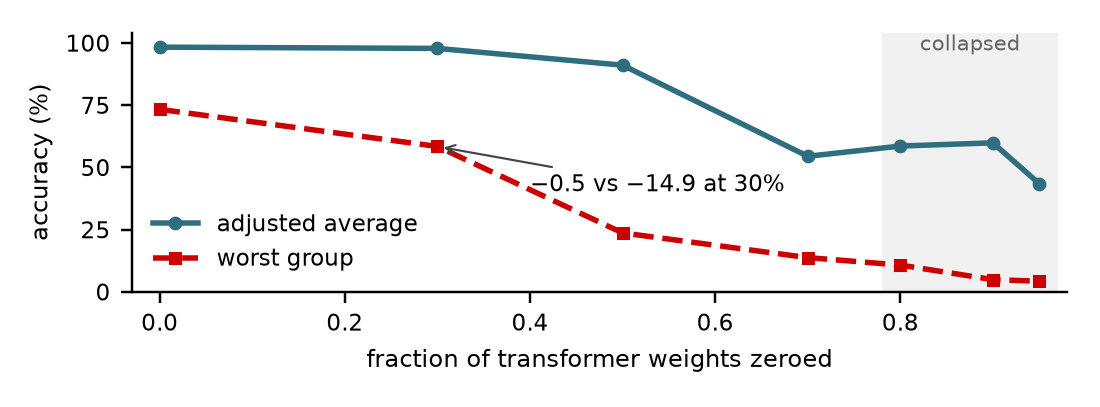
\includegraphics[width=0.66\textwidth]{figures/fig1_damage.png}
\caption{Average accuracy hides the damage: magnitude pruning, mean of 3
seeds. The gap opens from 30\% onward. Past 80\% individual seeds begin collapsing to
a single class, so neither curve is meaningful there.}
\label{fig:damage}
\end{figure}

Table~\ref{tab:phase1} gives the plain model. The dense checkpoint reaches
98.3\% adjusted average and 73.3\% worst group, a 25-point gap the shortcut
explains, and compression widens it in every family
(Figure~\ref{fig:damage}).

\begin{table}[t]
\centering
\small
\caption{Phase 1. A group-blind ViT-S/16 compressed four ways, mean of 3
seeds; deltas are against the uncompressed row.}
\label{tab:phase1}
\begin{tabular}{@{}lrrr@{}}
\toprule
Configuration & Achieved sparsity & Adjusted avg & Worst group \\
\midrule
uncompressed                & 0.000 & 98.3           & 73.3 \\
quantize 8-bit, per-channel & 0.014 & 98.3 ($+0.0$)  & 72.9 ($-0.4$) \\
quantize 6-bit, per-channel & 0.055 & 98.3 ($-0.1$)  & 74.2 ($+0.9$) \\
magnitude, 30\%             & 0.300 & 97.8 ($-0.5$)  & 58.4 ($\mathbf{-14.9}$) \\
quantize 4-bit, per-channel & 0.232 & 96.7 ($-1.6$)  & 66.7 ($-6.7$) \\
remove 6 of 72 heads        & 0.028 & 96.6 ($-1.7$)  & 55.1 ($\mathbf{-18.2}$) \\
FFN, 30\% of neurons        & 0.200 & 81.3 ($-17.1$) & 22.6 ($-50.7$) \\
\bottomrule
\end{tabular}
\end{table}

Read the magnitude row twice. Half a point of adjusted average against 14.9
points of worst group is the 29-to-one ratio, and nothing in a top-line
accuracy check would have caught it. Structured removal costs more per
parameter touched: 6 attention heads are 2.8\% of the targeted weights and
cost 18.2 points. The quantization scale matters more than the bit width, with
per-channel 4-bit keeping 66.7\% where per-tensor 4-bit keeps 8.0\%.

Past roughly 80\% sparsity the gap narrows again. Individual seeds are
collapsing to a single class by then, which leaves no disparity to measure.
Robustness is not coming back.

\subsection{The repair reproduces}

Across all nine arms the gain over ERM averages 13.9 points with a standard
deviation of 3.1 and is positive in every one. At the 50\% budget worst-group
accuracy rises from 73.3\% to 87.9\%, a gain of 14.6 points, and the gain is
flat from 25\% to 75\%, which is what the paper's Figure 8 claims.

\begin{table}[t]
\centering
\small
\caption{Phase 2, dense. Our budgets against ERM and the numbers published
by \citet{mulchandani2025severing}; Mean\% is the adjusted average, as in
that paper. Means over 3 seeds.}
\label{tab:phase2}
\begin{tabular}{@{}lrr@{}}
\toprule
 & Worst\% & Mean\% \\
\midrule
ERM, ours                  & 73.31 & 98.32 \\
ERM, published             & 74.81 & 98.10 \\
\midrule
delete 25\%                & 86.40 & 94.69 \\
delete 50\%                & \textbf{87.90} & 94.35 \\
delete 75\%                & 87.28 & 92.10 \\
published method           & 90.93 & 92.48 \\
\bottomrule
\end{tabular}
\end{table}

We land 3 points under the published 90.93, and we think the difficulty
ranking is why. Our backbone is pretrained and reaches 97.9\% training accuracy
after two passes, so the ranking has flattened by the time we score it; the
published setup trains from scratch for 100 epochs, where it still separates
samples. At the 50\% budget, 63\% of what we delete is material the model
already classifies above 99.3\% confidence, and 65\% and 64\% at the other two
budgets. Our version mostly shrinks and balances the training set rather than
removing hard samples, so 14.6 should be read as a lower bound on the method.

\subsection{What predicts retention}

We built the sweep expecting $R$ to differ by compression family, since Phase
1 had just shown the families are not interchangeable. It does not. What
predicts $R$ is whether compression left a model that works at all
(Table~\ref{tab:retention}).

\begin{table}[t]
\centering
\small
\caption{Retention across the 168 compressed non-collapsed configurations,
bucketed by the compressed model's own worst-group accuracy. The 27
uncompressed rows are excluded: $R(0) = 1$ by construction.}
\label{tab:retention}
\begin{tabular}{@{}lrrr@{}}
\toprule
Regime & $n$ & mean $R$ & $R \geq 0.75$ \\
\midrule
compressed worst group $\geq 0.40$ (usable) & 87  & $+1.39$ & 95\% \\
$0.25$ to $0.40$ (degraded)                 & 14  & $+1.30$ & 86\% \\
below $0.25$ (broken)                       & 67  & $-0.20$ & 13\% \\
\bottomrule
\end{tabular}
\end{table}

We bucket by the compressed model's own worst-group accuracy at 0.40 and 0.25;
moving either cutoff by 0.05 leaves the usable and broken buckets essentially
unchanged. Inside the usable regime $R$ runs from $+0.29$ to $+3.58$ across all
four families, and negative values never appear above a compressed worst-group
accuracy of 0.269. A mean $R$ above one says the gap usually widens. At 50\%
magnitude sparsity the plain model loses 49.6 points of worst-group accuracy
and the repaired model loses 34.9, so $D$ doubles and $R$ reaches 2.04.

\subsection{Why $R$ goes negative}

Worst-group accuracy is a minimum over four groups and says nothing about which
group is binding. Breaking the gain out per group (Table~\ref{tab:pergroup})
shows the targeted group still benefiting long after worst-group accuracy stops
reporting it (Figure~\ref{fig:pergroup}).

\begin{table}[t]
\centering
\small
\caption{Per-group gain of the repaired model over the plain one, magnitude
pruning on the delete 50\% arm, mean of 3 seeds, in points. The last column
gives the binding group of the plain model $\rightarrow$ that of the repaired
one. At 70\% the worst-group column reads $-0.4$ while g2 is 21 points ahead.}
\label{tab:pergroup}
\begin{tabular}{@{}lrrrrrc@{}}
\toprule
Sparsity & g0 & g1 & \textbf{g2} & g3 & worst group & binding group \\
\midrule
30\% & $-3.8$  & $+3.7$  & $\mathbf{+23.5}$ & $-7.1$ & $+23.5$ & g2 $\rightarrow$ g2 \\
50\% & $-17.2$ & $+5.0$  & $\mathbf{+33.5}$ & $-1.0$ & $+29.4$ & g2 $\rightarrow$ g2 \\
70\% & $-19.1$ & $-11.4$ & $\mathbf{+21.0}$ & $+11.0$ & $-0.4$ & g2 $\rightarrow$ \textbf{g0} \\
\bottomrule
\end{tabular}
\end{table}

\begin{figure}[t]
\centering
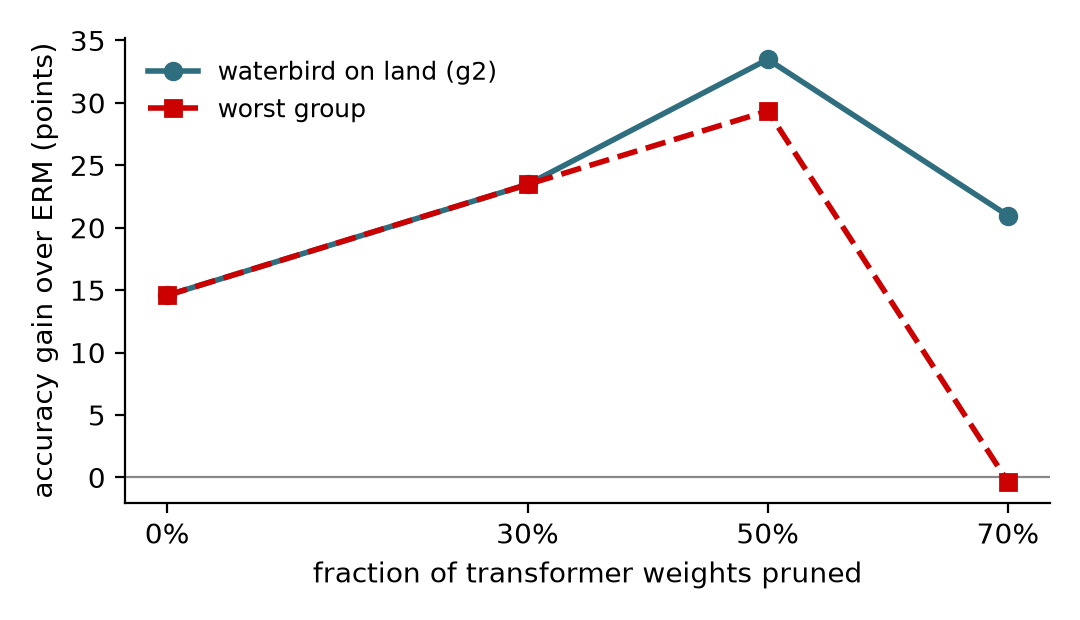
\includegraphics[width=0.56\textwidth]{figures/fig4_per_group_retention.png}
\caption{Where worst-group accuracy stops tracking the repair. Gain of the
repaired model over the plain one, magnitude pruning on the delete 50\% arm,
mean of 3 seeds. The curves coincide up to 30\% and separate from 50\% on; at 70\% the worst-group gain has fallen to $-0.4$ while waterbird-on-land is 21 points ahead,
because the binding group has moved to the majority group.}
\label{fig:pergroup}
\end{figure}

At 70\% sparsity the binding group moves to landbird-on-land, the majority
group, which has nothing to do with the spurious correlation. Worst-group
accuracy reports $-0.4$ points for a model that is 21 points better on the
group the repair was aimed at.

Splitting the 168 settings where $R$ is defined by its sign makes this
quantitative. Where $R < 0$ ($n = 43$) the worst-group gain averages $-9.0$
points, while the gain on waterbird-on-land averages $+21.9$ and is positive in
34 of those 43 runs. Where $R \geq 0$ ($n = 125$) the two figures are $+17.6$
and $+20.8$. The effect on the group the repair targets is the same in both
halves to within a point and a half. What changes is whether worst-group
accuracy is still pointing at that group: the repaired model's worst group is
no longer waterbird-on-land in 93\% of negative-$R$ settings against 50\% of
the rest, and has left both counter-shortcut groups in 35\% against 18\%.

So a negative $R$ mostly does not mean the repair was destroyed. It means
worst-group accuracy moved once compression broke the majority group badly
enough to make it the minimum. Report which group is binding next to the
number.

\subsection{What went wrong}

Three bugs changed numbers we had already written down, and one killed a
planned experiment.

The sweep resumes by skipping configurations already in \texttt{sweep.csv},
and a row's identity was originally \texttt{(method, param\_value,
granularity)}. Seed 1 matched every row seed 0 had written, declared all 29
configurations done and exited having computed nothing. The identity now
carries the tag, seed and checkpoint. Second, \texttt{-{}-stop-after-epoch} scores difficulty without writing a
selection checkpoint, but its break test sat after the save test, so epoch 0
of a \texttt{score\_epoch: 1} run fell through and overwrote
\texttt{vit\_s16\_waterbirds\_seed0.pt} with epoch-0 weights, 0.8616
validation accuracy against 0.9199. Checkpoints are gitignored and were not
backed up, so we retrained. Third, our own Table~\ref{tab:retention} was wrong
in an earlier draft: we bucketed all 195 non-collapsed rows, 27 of which are
the uncompressed setting where $R(0) = 1$ by construction. They all landed in
the usable bucket. Dropping them moves that row from 114 settings at a mean
$R$ of 1.30 to 87 at 1.39.

The proposal specified budgets of $\{1, 2, 5, 10\}\%$. Twelve of those arms
died partway through the sweep with \texttt{Errno 28: No space left on
device}, the uint8 caches having filled the disk, and rather than re-run them
we moved to the 25/50/75\% budgets the paper itself sweeps. We also lost a
night to a machine that slept mid-run: epoch 8 of seed 0 took 3338 seconds
against 114 for every uninterrupted epoch.

\section{Conclusion and limitations}

The thing we would change first is the difficulty score. Scoring a pretrained
backbone at epoch 1 gives a ranking that has already flattened, and that is
the most likely reason we land 3 points short of the published method. A
longer schedule, or scoring from a randomly initialized head, would test it
directly.

Four limits are worth stating. This is one dataset and one architecture, and
Waterbirds has a clean synthetic shortcut that natural distribution shift does
not. Head and neuron importance is weight norm with no calibration data, and a
data-aware criterion might prune in a more robustness-preserving order. Phase
1 reports means over three seeds with no spread, and worst-group accuracy on a
642-image group moves around; the Phase 2 gain carries a standard deviation of
3.1 for that reason, and Phase 1 should carry one too. Finally, $R$ inherits every weakness of worst-group accuracy, and we have
shown it can report a loss for a model that improved on the group the repair
targeted.

\section*{Contribution of each member}

\begin{table}[H]
\centering
\footnotesize
\begin{tabular}{@{}>{\raggedright\arraybackslash}p{0.20\textwidth}p{0.755\textwidth}@{}}
\toprule
\textbf{Shreyas Visweshwaran} \texttt{sviswes}
& All four compression families behind one \texttt{apply} contract, with
exact structured removal; the frozen 21.2M-weight scope; the Phase 1 sweep. \\
\addlinespace
\textbf{Swasti Sadanand} \texttt{ssadana}
& The Phase 2 data pruning and both selection rules; the retention ratio $R$,
the rule leaving it undefined when the dense gain is within noise, and the
usability buckets; the comparison against the published result. \\
\addlinespace
\textbf{Anusha Upadhyay} \texttt{aupadhy6}
& Group indexing, per-group and adjusted-average accuracy, the collapse gate;
64 automated tests and 15 shell checks; the figures and tables. \\
\bottomrule
\end{tabular}
\end{table}

\setlength{\bibsep}{0pt plus 0.3ex}
{\footnotesize\bibliography{refs}}

\end{document}
